\begin{frame}
  \frametitle{Influence diagnostics for MLMs}

  \begin{itemize}
  \item<1-> Influence measures and diagnostic plots are well-developed for univariate LMs
    \begin{itemize}
    \item Influence measures: Cook's D, DFFITS, dfbetas, etc.
    \item Diagnostic plots:  Index plots, \code{car:::influencePlot()} for LMs
    \item However, these are have been unavailable for MLMs  
    \end{itemize}
  \item<2->
    The \package{mvinfluence} now provides:
    \begin{itemize}
    \item Calculation for multivariate analogs of univariate influence measures
    (following Barrett \& Ling, 1992), e.g., Hat values \& Cook's $D$:
    \begin{equation}
    	H_I = \mat{X}_I
    	      (\mat{X}\trans\mat{X})^{-1}
    	      \mat{X}_I\trans
    \end{equation}
    \begin{equation}
    	D_I = [vec(\mat{B} - \mat{B}_{(I)})]\trans
    	      [\mat{S}^{-1} \otimes (\mat{X}\trans\mat{X})]
    	      [vec(\mat{B} - \mat{B}_{(I)})]
    \end{equation}
    \item Provides deletion diagnostics for subsets $(I)$ of size $m \ge 1$.
    \item e.g., $m=2$ can reveal cases of \alert{masking} or \alert{joint influence}.
    \item Extension of \code{influencePlot()} to the multivariate case.
    \item A new plot format: \alert{leverage-residual (LR) plots}.
    \end{itemize}
  \end{itemize}
\end{frame}

\begin{frame}
  \frametitle{Influence diagnostics for MLMs: Example}
  For the Rohwer data:

% two figs side-by-side
  \begin{minipage}[c]{.5\textwidth}
   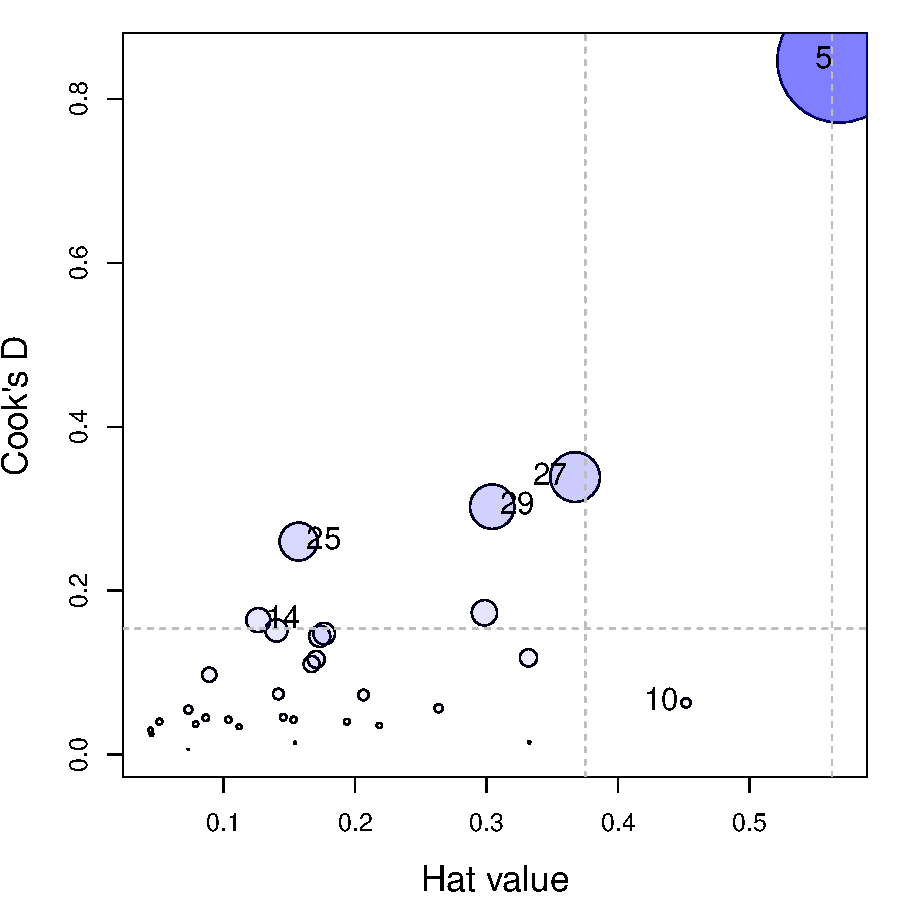
\includegraphics[width=1\linewidth,clip]{figures/rohwer-influence-cookd}
   \\ \centering Cook's $D$ vs. generalized Hat value
   \end{minipage}%
  \hfill
  \begin{minipage}[c]{.5\textwidth}
   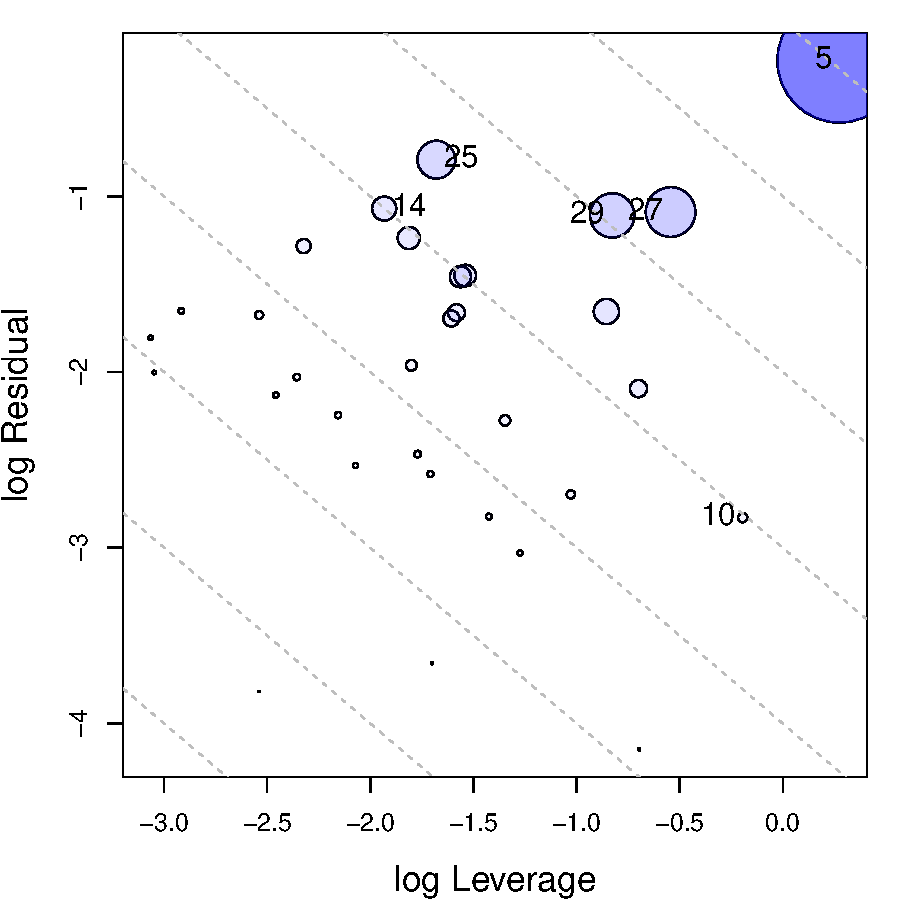
\includegraphics[width=1\linewidth,clip]{figures/rohwer-influence-LR}
   \\ \centering Leverage - Residual (LR) plot
  \end{minipage}

\end{frame}

\begin{frame}
  \frametitle{Influence diagnostics for MLMs: LR plots}

  \begin{columns}[T]
    \begin{column}{.5\textwidth}
	  \begin{itemize}
	    \item Main idea: Influence $\sim$ Leverage (L) $\times$ Residual (R)
			\item $\implies \log (Infl) = \log(L) + \log(R)$
			\item $\implies$ contours of constant influence 
			lie on lines with slope = -1.
			\item Bubble size $\sim$ influence (Cook's $D$)
			\item This simplifies interpretation of influence measures
	  \end{itemize}
    \end{column}
    \begin{column}{.5\textwidth}
    \includegraphics<1>[width=\textwidth,clip]{figures/rohwer-influence-LR}
    \end{column}
  \end{columns}

\end{frame}
